% Options for packages loaded elsewhere
\PassOptionsToPackage{unicode}{hyperref}
\PassOptionsToPackage{hyphens}{url}
\PassOptionsToPackage{dvipsnames,svgnames*,x11names*}{xcolor}
%
\documentclass[
  10pt,
  ignorenonframetext,
]{beamer}
\usepackage{pgfpages}
\setbeamertemplate{caption}[numbered]
\setbeamertemplate{caption label separator}{: }
\setbeamercolor{caption name}{fg=normal text.fg}
\beamertemplatenavigationsymbolsempty
% Prevent slide breaks in the middle of a paragraph
\widowpenalties 1 10000
\raggedbottom
\setbeamertemplate{part page}{
  \centering
  \begin{beamercolorbox}[sep=16pt,center]{part title}
    \usebeamerfont{part title}\insertpart\par
  \end{beamercolorbox}
}
\setbeamertemplate{section page}{
  \centering
  \begin{beamercolorbox}[sep=12pt,center]{part title}
    \usebeamerfont{section title}\insertsection\par
  \end{beamercolorbox}
}
\setbeamertemplate{subsection page}{
  \centering
  \begin{beamercolorbox}[sep=8pt,center]{part title}
    \usebeamerfont{subsection title}\insertsubsection\par
  \end{beamercolorbox}
}
\AtBeginPart{
  \frame{\partpage}
}
\AtBeginSection{
  \ifbibliography
  \else
    \frame{\sectionpage}
  \fi
}
\AtBeginSubsection{
  \frame{\subsectionpage}
}
\usepackage{lmodern}
\usepackage{amssymb,amsmath}
\usepackage{ifxetex,ifluatex}
\ifnum 0\ifxetex 1\fi\ifluatex 1\fi=0 % if pdftex
  \usepackage[T1]{fontenc}
  \usepackage[utf8]{inputenc}
  \usepackage{textcomp} % provide euro and other symbols
\else % if luatex or xetex
  \usepackage{unicode-math}
  \defaultfontfeatures{Scale=MatchLowercase}
  \defaultfontfeatures[\rmfamily]{Ligatures=TeX,Scale=1}
\fi
\usetheme[]{AnnArbor}
\usecolortheme{dolphin}
\usefonttheme{structurebold}
% Use upquote if available, for straight quotes in verbatim environments
\IfFileExists{upquote.sty}{\usepackage{upquote}}{}
\IfFileExists{microtype.sty}{% use microtype if available
  \usepackage[]{microtype}
  \UseMicrotypeSet[protrusion]{basicmath} % disable protrusion for tt fonts
}{}
\makeatletter
\@ifundefined{KOMAClassName}{% if non-KOMA class
  \IfFileExists{parskip.sty}{%
    \usepackage{parskip}
  }{% else
    \setlength{\parindent}{0pt}
    \setlength{\parskip}{6pt plus 2pt minus 1pt}}
}{% if KOMA class
  \KOMAoptions{parskip=half}}
\makeatother
\usepackage{xcolor}
\IfFileExists{xurl.sty}{\usepackage{xurl}}{} % add URL line breaks if available
\IfFileExists{bookmark.sty}{\usepackage{bookmark}}{\usepackage{hyperref}}
\hypersetup{
  pdftitle={Forecast financial crisis in brasilian stock market using Naive Bayes},
  pdfauthor={Marcos J Ribeiro},
  colorlinks=true,
  linkcolor=Maroon,
  filecolor=Maroon,
  citecolor=Blue,
  urlcolor=blue,
  pdfcreator={LaTeX via pandoc}}
\urlstyle{same} % disable monospaced font for URLs
\newif\ifbibliography
\usepackage{color}
\usepackage{fancyvrb}
\newcommand{\VerbBar}{|}
\newcommand{\VERB}{\Verb[commandchars=\\\{\}]}
\DefineVerbatimEnvironment{Highlighting}{Verbatim}{commandchars=\\\{\}}
% Add ',fontsize=\small' for more characters per line
\usepackage{framed}
\definecolor{shadecolor}{RGB}{248,248,248}
\newenvironment{Shaded}{\begin{snugshade}}{\end{snugshade}}
\newcommand{\AlertTok}[1]{\textcolor[rgb]{0.94,0.16,0.16}{#1}}
\newcommand{\AnnotationTok}[1]{\textcolor[rgb]{0.56,0.35,0.01}{\textbf{\textit{#1}}}}
\newcommand{\AttributeTok}[1]{\textcolor[rgb]{0.77,0.63,0.00}{#1}}
\newcommand{\BaseNTok}[1]{\textcolor[rgb]{0.00,0.00,0.81}{#1}}
\newcommand{\BuiltInTok}[1]{#1}
\newcommand{\CharTok}[1]{\textcolor[rgb]{0.31,0.60,0.02}{#1}}
\newcommand{\CommentTok}[1]{\textcolor[rgb]{0.56,0.35,0.01}{\textit{#1}}}
\newcommand{\CommentVarTok}[1]{\textcolor[rgb]{0.56,0.35,0.01}{\textbf{\textit{#1}}}}
\newcommand{\ConstantTok}[1]{\textcolor[rgb]{0.00,0.00,0.00}{#1}}
\newcommand{\ControlFlowTok}[1]{\textcolor[rgb]{0.13,0.29,0.53}{\textbf{#1}}}
\newcommand{\DataTypeTok}[1]{\textcolor[rgb]{0.13,0.29,0.53}{#1}}
\newcommand{\DecValTok}[1]{\textcolor[rgb]{0.00,0.00,0.81}{#1}}
\newcommand{\DocumentationTok}[1]{\textcolor[rgb]{0.56,0.35,0.01}{\textbf{\textit{#1}}}}
\newcommand{\ErrorTok}[1]{\textcolor[rgb]{0.64,0.00,0.00}{\textbf{#1}}}
\newcommand{\ExtensionTok}[1]{#1}
\newcommand{\FloatTok}[1]{\textcolor[rgb]{0.00,0.00,0.81}{#1}}
\newcommand{\FunctionTok}[1]{\textcolor[rgb]{0.00,0.00,0.00}{#1}}
\newcommand{\ImportTok}[1]{#1}
\newcommand{\InformationTok}[1]{\textcolor[rgb]{0.56,0.35,0.01}{\textbf{\textit{#1}}}}
\newcommand{\KeywordTok}[1]{\textcolor[rgb]{0.13,0.29,0.53}{\textbf{#1}}}
\newcommand{\NormalTok}[1]{#1}
\newcommand{\OperatorTok}[1]{\textcolor[rgb]{0.81,0.36,0.00}{\textbf{#1}}}
\newcommand{\OtherTok}[1]{\textcolor[rgb]{0.56,0.35,0.01}{#1}}
\newcommand{\PreprocessorTok}[1]{\textcolor[rgb]{0.56,0.35,0.01}{\textit{#1}}}
\newcommand{\RegionMarkerTok}[1]{#1}
\newcommand{\SpecialCharTok}[1]{\textcolor[rgb]{0.00,0.00,0.00}{#1}}
\newcommand{\SpecialStringTok}[1]{\textcolor[rgb]{0.31,0.60,0.02}{#1}}
\newcommand{\StringTok}[1]{\textcolor[rgb]{0.31,0.60,0.02}{#1}}
\newcommand{\VariableTok}[1]{\textcolor[rgb]{0.00,0.00,0.00}{#1}}
\newcommand{\VerbatimStringTok}[1]{\textcolor[rgb]{0.31,0.60,0.02}{#1}}
\newcommand{\WarningTok}[1]{\textcolor[rgb]{0.56,0.35,0.01}{\textbf{\textit{#1}}}}
\usepackage{longtable,booktabs}
\usepackage{caption}
% Make caption package work with longtable
\makeatletter
\def\fnum@table{\tablename~\thetable}
\makeatother
\usepackage{graphicx,grffile}
\makeatletter
\def\maxwidth{\ifdim\Gin@nat@width>\linewidth\linewidth\else\Gin@nat@width\fi}
\def\maxheight{\ifdim\Gin@nat@height>\textheight\textheight\else\Gin@nat@height\fi}
\makeatother
% Scale images if necessary, so that they will not overflow the page
% margins by default, and it is still possible to overwrite the defaults
% using explicit options in \includegraphics[width, height, ...]{}
\setkeys{Gin}{width=\maxwidth,height=\maxheight,keepaspectratio}
% Set default figure placement to htbp
\makeatletter
\def\fps@figure{htbp}
\makeatother
\setlength{\emergencystretch}{3em} % prevent overfull lines
\providecommand{\tightlist}{%
  \setlength{\itemsep}{0pt}\setlength{\parskip}{0pt}}
\setcounter{secnumdepth}{-\maxdimen} % remove section numbering

\title{Forecast financial crisis in brasilian stock market using Naive Bayes}
\author{Marcos J Ribeiro}
\date{19/05/2020}
\institute{FEARP-USP}

\begin{document}
\frame{\titlepage}

\begin{frame}{My Machine Learning work}
\protect\hypertarget{my-machine-learning-work}{}

\begin{itemize}
\item
  I built Naive Bayes algorithm to solve classification problems
\item
  I used R language, version 4.0, to do this
\item
  This presentation was built using Beamer Rmarkdown
\item
  My Naive Bayes algorithm and this presentation can be view in my
  \href{https://github.com/mj-ribeiro/College-works/tree/master/ML_1}{Github}.
  This presentation can also be seen in my
  \href{https://rpubs.com/mj-ribeiro/616774}{Rpubs}
\item
  First, i will apply my algorithm in four data sets. The first two are
  simple
\item
  After, i will apply my algorithm in brasilian stock market to
  identified crisis. This is my principal analysis
\item
  I will try to predict the crash of brasilian stock market during
  COVID-19 pandemic
\item
  There are two types of independent variables: Categorical and
  non-categorical
\item
  The approach to classification in this context is diferent
\item
  So, i built two functions to solve this, and put this two functions
  inside one
\end{itemize}

\end{frame}

\begin{frame}[fragile]{Naive Bayes function}
\protect\hypertarget{naive-bayes-function}{}

\begin{itemize}
\tightlist
\item
  I created two functions: one to be used in datasets with categorical
  independent variables and the other to be used in datasets with
  non-categorical independent variables
\end{itemize}

\begin{Shaded}
\begin{Highlighting}[]
\NormalTok{naivef =}\StringTok{ }\ControlFlowTok{function}\NormalTok{(k, df, }\DataTypeTok{cd=}\DecValTok{1}\NormalTok{)\{}
    \ControlFlowTok{if}\NormalTok{(cd }\OperatorTok{==}\StringTok{ }\DecValTok{1}\NormalTok{)\{}
      \KeywordTok{naive_marcos}\NormalTok{(k, df)}
\NormalTok{    \}}\ControlFlowTok{else} \ControlFlowTok{if}\NormalTok{ (cd }\OperatorTok{==}\StringTok{ }\DecValTok{0}\NormalTok{)\{}
      \KeywordTok{naive_marcos2}\NormalTok{(k, df)}
\NormalTok{    \}}\ControlFlowTok{else}\NormalTok{\{}
      \KeywordTok{cat}\NormalTok{(}\StringTok{'Type cd = 1 for categorical dependent variables, }\CharTok{\textbackslash{}n}
\StringTok{      and cd = 0 for non-categorical dependent variables.'}\NormalTok{)}
\NormalTok{    \}\} }
\end{Highlighting}
\end{Shaded}

\begin{itemize}
\tightlist
\item
  If cd=1 the algorithm can be used in classification problems with
  categorical dependent variables (naive\_marcos)
\item
  If cd=0 the algorithm can be used in classification problems with
  non-categorical dependent variables (naive\_marcos2)
\end{itemize}

\end{frame}

\begin{frame}[fragile]{Naive Bayes function}
\protect\hypertarget{naive-bayes-function-1}{}

\begin{itemize}
\tightlist
\item
  k is the class
\item
  df is the data frame that contains the dataset of interest
\item
  My predict function can be see below
\end{itemize}

\begin{Shaded}
\begin{Highlighting}[]
\NormalTok{predf =}\StringTok{ }\ControlFlowTok{function}\NormalTok{(k, df, df_n, cl, }\DataTypeTok{cclas=}\DecValTok{0}\NormalTok{, }\DataTypeTok{cd=}\DecValTok{1}\NormalTok{)\{}
  \ControlFlowTok{if}\NormalTok{(cd }\OperatorTok{==}\StringTok{ }\DecValTok{1}\NormalTok{)\{}
    \KeywordTok{pred_marcos}\NormalTok{(k, df, df_n, cl, cclas)}
\NormalTok{  \}}\ControlFlowTok{else} \ControlFlowTok{if}\NormalTok{ (cd }\OperatorTok{==}\StringTok{ }\DecValTok{0}\NormalTok{)\{}
    \KeywordTok{pred_marcos2}\NormalTok{(k, df, df_n, cl, cclas)}
\NormalTok{  \}}\ControlFlowTok{else}\NormalTok{\{}
    \KeywordTok{cat}\NormalTok{(}\StringTok{'Type cd = 1 for categorical dependent variables, }
\StringTok{    }\CharTok{\textbackslash{}n}\StringTok{ and cd = 0 for non-categorical dependent variables.'}\NormalTok{)}
\NormalTok{  \}\} }
\end{Highlighting}
\end{Shaded}

\begin{itemize}
\tightlist
\item
  df\_n is the new data set that we want to predict the class
\item
  cl is the inductor
\item
  cclas gives the class if cclas=1, and probabilities if cclas=0
\end{itemize}

\end{frame}

\begin{frame}{My first example (default risk)}
\protect\hypertarget{my-first-example-default-risk}{}

\begin{itemize}
\tightlist
\item
  There are three attributes in dependent variable (risco) and two
  independents variables. The independent variables (historia, divida)
  are categoricals as you can see in head table of my data set:
\end{itemize}

\begin{longtable}[]{@{}lll@{}}
\caption{Dataset with categorical independent variables}\tabularnewline
\toprule
historia & divida & risco\tabularnewline
\midrule
\endfirsthead
\toprule
historia & divida & risco\tabularnewline
\midrule
\endhead
ruim & alta & alto\tabularnewline
desconhecida & alta & alto\tabularnewline
desconhecida & baixa & moderado\tabularnewline
desconhecida & baixa & alto\tabularnewline
desconhecida & baixa & baixo\tabularnewline
desconhecida & baixa & baixo\tabularnewline
\bottomrule
\end{longtable}

\begin{itemize}
\tightlist
\item
  Risco is a default risk that the bank runs when lending money
\item
  Historia is customer credit history and divida is customer debt in
  market\\
\item
  So, I will predict if the new customer is a good customer
\end{itemize}

\end{frame}

\begin{frame}{Plots}
\protect\hypertarget{plots}{}

\begin{itemize}
\tightlist
\item
  I use ggplot to plot my data set.
\item
  Note that credit history is important to predict risk default
\end{itemize}

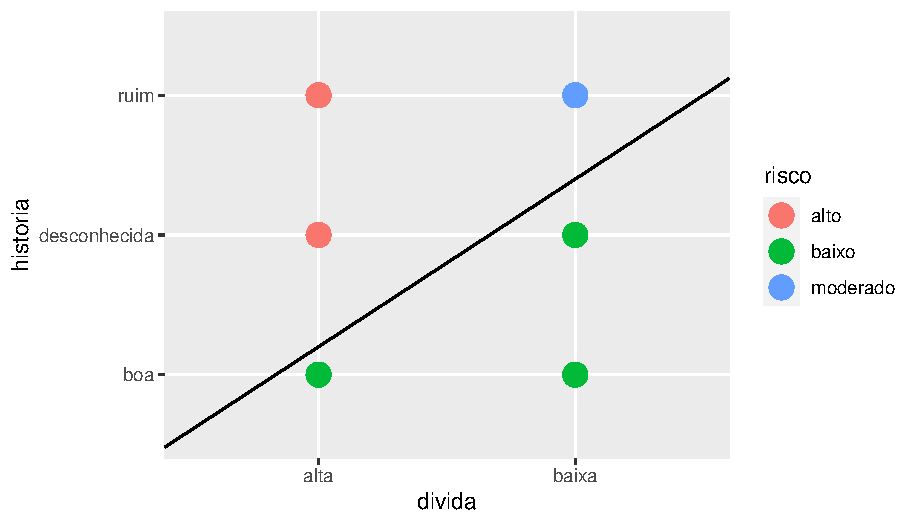
\includegraphics{MJ_Ribeiro_files/figure-beamer/unnamed-chunk-5-1.pdf}

\end{frame}

\begin{frame}[fragile]{Inductor to categorical dependet variables}
\protect\hypertarget{inductor-to-categorical-dependet-variables}{}

\begin{itemize}
\tightlist
\item
  I used naivef function in my dataset
\end{itemize}

\begin{Shaded}
\begin{Highlighting}[]
\NormalTok{cl =}\StringTok{ }\KeywordTok{naivef}\NormalTok{(}\StringTok{'risco'}\NormalTok{, df, }\DataTypeTok{cd=}\DecValTok{1}\NormalTok{)}
\end{Highlighting}
\end{Shaded}

\begin{verbatim}
## [1] "=-=-=-=-=-=-=-=-=-=-=-=-=-=-=-=-=-=-=-=-=-=-=-=-=-=-=-"
## [1] "Marcos Naive Bayes Classifier for Discrete Predictors"
## [1] "=-=-=-=-=-=-=-=-=-=-=-=-=-=-=-=-=-=-=-=-=-=-=-=-=-=-=-"
## A-priori probabilities:
## 
##      alto     baixo  moderado 
## 0.4285714 0.3571429 0.2142857 
## Conditional Probabilities:
\end{verbatim}

\begin{itemize}
\tightlist
\item
  This function return a table that contains conditional probabilities
\item
  This table was save in cl object
\end{itemize}

\end{frame}

\begin{frame}[fragile]{Inductor to categorical dependet variables}
\protect\hypertarget{inductor-to-categorical-dependet-variables-1}{}

\begin{itemize}
\tightlist
\item
  cl object is a tensor
\item
  The tensor has a dimension equal to the number of the class
  attributes. In this case three
\item
  You can see below the first dimension of this tensor
\item
  The first row of first column is: \[P(alta, boa|alto)= 0.04761\]
\end{itemize}

\begin{Shaded}
\begin{Highlighting}[]
\KeywordTok{head}\NormalTok{(cl[, ,}\DecValTok{1}\NormalTok{])}
\end{Highlighting}
\end{Shaded}

\begin{verbatim}
##                    alta      baixa
## boa          0.04761905 0.02380952
## desconhecida 0.09523810 0.04761905
## ruim         0.14285714 0.07142857
\end{verbatim}

\end{frame}

\begin{frame}{Predict}
\protect\hypertarget{predict}{}

\begin{itemize}
\tightlist
\item
  I have six new customers and i want to know if they are good payers
\item
  My new data set can be see below
\end{itemize}

\begin{longtable}[]{@{}ll@{}}
\caption{New data set with categorical independent
variables}\tabularnewline
\toprule
historia & divida\tabularnewline
\midrule
\endfirsthead
\toprule
historia & divida\tabularnewline
\midrule
\endhead
boa & baixa\tabularnewline
boa & alta\tabularnewline
ruim & baixa\tabularnewline
ruim & alta\tabularnewline
desconhecida & baixa\tabularnewline
desconhecida & alta\tabularnewline
\bottomrule
\end{longtable}

\begin{itemize}
\tightlist
\item
  To do this i used predf function
\end{itemize}

\end{frame}

\begin{frame}[fragile]{Predict}
\protect\hypertarget{predict-1}{}

\begin{itemize}
\tightlist
\item
  Here, i used cclas = 0, so, my function return the probabilities of
  risk associated with my new client
\end{itemize}

\begin{Shaded}
\begin{Highlighting}[]
\KeywordTok{predf}\NormalTok{(}\StringTok{'risco'}\NormalTok{, df, df_teste, cl, }\DataTypeTok{cclas =} \DecValTok{0}\NormalTok{, }\DataTypeTok{cd=}\DecValTok{1}\NormalTok{)}
\end{Highlighting}
\end{Shaded}

\begin{verbatim}
##           alto     baixo  moderado
## [1,] 0.1190476 0.6428571 0.2380952
## [2,] 0.3030303 0.5454545 0.1515152
## [3,] 0.6000000 0.0000000 0.4000000
## [4,] 0.8571429 0.0000000 0.1428571
## [5,] 0.2631579 0.4736842 0.2631579
## [6,] 0.5405405 0.3243243 0.1351351
\end{verbatim}

\end{frame}

\begin{frame}[fragile]{Predict}
\protect\hypertarget{predict-2}{}

\begin{itemize}
\tightlist
\item
  Here, i used cclas = 1, so, my function return the attribute of my new
  client
\item
  Recall that cd=1 is to categorical independent variables
\end{itemize}

\begin{Shaded}
\begin{Highlighting}[]
\KeywordTok{predf}\NormalTok{(}\StringTok{'risco'}\NormalTok{, df, df_teste, cl, }\DataTypeTok{cclas =} \DecValTok{1}\NormalTok{, }\DataTypeTok{cd=}\DecValTok{1}\NormalTok{)}
\end{Highlighting}
\end{Shaded}

\begin{verbatim}
## [1] "baixo" "baixo" "alto"  "alto"  "baixo" "alto"
\end{verbatim}

\end{frame}

\begin{frame}[fragile]{Quality control}
\protect\hypertarget{quality-control}{}

\begin{itemize}
\tightlist
\item
  Here only to verify if my algorith is correct i compared to Naive
  Bayes produced by library e1071
\end{itemize}

\begin{Shaded}
\begin{Highlighting}[]
\KeywordTok{library}\NormalTok{(e1071) }
\NormalTok{clas2 =}\StringTok{ }\KeywordTok{naiveBayes}\NormalTok{(}\DataTypeTok{x=}\NormalTok{df[}\OperatorTok{-}\DecValTok{3}\NormalTok{], }\DataTypeTok{y =} \KeywordTok{as.factor}\NormalTok{(df}\OperatorTok{$}\NormalTok{risco))}
\NormalTok{prev2 =}\StringTok{ }\KeywordTok{predict}\NormalTok{(clas2, }\DataTypeTok{newdata =}\NormalTok{ df_teste) }
\KeywordTok{print}\NormalTok{(prev2) }
\end{Highlighting}
\end{Shaded}

\begin{verbatim}
## [1] baixo baixo alto  alto  baixo alto 
## Levels: alto baixo moderado
\end{verbatim}

\begin{itemize}
\tightlist
\item
  The answers of my algorithm and e1071 are identical
\end{itemize}

\end{frame}

\begin{frame}{My second example}
\protect\hypertarget{my-second-example}{}

\begin{itemize}
\tightlist
\item
  I have two attributes in dependent variable (sex) and two independent
  variables, weight and height
\item
  Weight and height are non-categorical as you can see in head table of
  my data set
\end{itemize}

\begin{longtable}[]{@{}rrl@{}}
\caption{Data set with non categorical independent
variables}\tabularnewline
\toprule
height & weight & sex\tabularnewline
\midrule
\endfirsthead
\toprule
height & weight & sex\tabularnewline
\midrule
\endhead
6.00 & 180 & male\tabularnewline
5.92 & 190 & male\tabularnewline
5.58 & 170 & male\tabularnewline
5.92 & 165 & male\tabularnewline
5.00 & 100 & female\tabularnewline
5.50 & 150 & female\tabularnewline
\bottomrule
\end{longtable}

\begin{itemize}
\tightlist
\item
  Height and weight are characteristics of the individual
\item
  And i will predict your sex based in this variables
\end{itemize}

\end{frame}

\begin{frame}{Plots}
\protect\hypertarget{plots-1}{}

\begin{itemize}
\tightlist
\item
  I use ggplot to plot my data set. Note that male is havier than female
\item
  And on average, the man is taller
  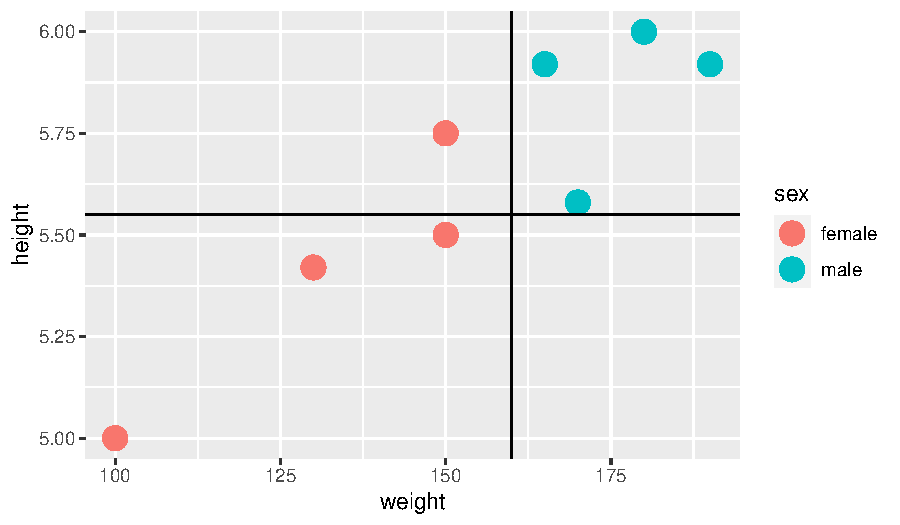
\includegraphics{MJ_Ribeiro_files/figure-beamer/unnamed-chunk-13-1.pdf}
\end{itemize}

\end{frame}

\begin{frame}[fragile]{Inductor to non-categorical dependet variables}
\protect\hypertarget{inductor-to-non-categorical-dependet-variables}{}

\begin{Shaded}
\begin{Highlighting}[]
\NormalTok{cl2 =}\StringTok{ }\KeywordTok{naivef}\NormalTok{(}\StringTok{'sex'}\NormalTok{, teste, }\DataTypeTok{cd=}\DecValTok{0}\NormalTok{)}
\end{Highlighting}
\end{Shaded}

\begin{verbatim}
## [1] "=-=-=-=-=-=-=-=-=-=-=-=-=-=-=-=-=-=-=-=-=-=-=-=-=-=-=-"
## [1] "Marcos Naive Bayes Classifier for Discrete Predictors"
## [1] "=-=-=-=-=-=-=-=-=-=-=-=-=-=-=-=-=-=-=-=-=-=-=-=-=-=-=-"
## A-priori probabilities:
## 
## female   male 
##    0.5    0.5
\end{verbatim}

\begin{itemize}
\tightlist
\item
  This function return a table that contains conditional probabilities
\item
  This table was save in cl2 object
\end{itemize}

\end{frame}

\begin{frame}[fragile]{Inductor to non-categorical dependet variables}
\protect\hypertarget{inductor-to-non-categorical-dependet-variables-1}{}

\begin{itemize}
\tightlist
\item
  cl2 is a tensor that contains the two first moments of height and
  weight by sex. As you can see below
\item
  The tensor has a dimension equal to the number of the class attributes
\end{itemize}

\begin{Shaded}
\begin{Highlighting}[]
\NormalTok{cl2}
\end{Highlighting}
\end{Shaded}

\begin{verbatim}
## , , female
## 
##          mean   variance
## [1,]   5.4175  0.3118092
## [2,] 132.5000 23.6290781
## 
## , , male
## 
##         mean   variance
## [1,]   5.855  0.1871719
## [2,] 176.250 11.0867789
\end{verbatim}

\end{frame}

\begin{frame}{Predict}
\protect\hypertarget{predict-3}{}

\begin{itemize}
\tightlist
\item
  I have four new people and i want to know if they are male or female
\item
  My new data set can be see below
\end{itemize}

\begin{longtable}[]{@{}rr@{}}
\caption{New data set with non categorical independent
variables}\tabularnewline
\toprule
height & weight\tabularnewline
\midrule
\endfirsthead
\toprule
height & weight\tabularnewline
\midrule
\endhead
5.4 & 170\tabularnewline
5.8 & 183\tabularnewline
6.0 & 188\tabularnewline
5.0 & 188\tabularnewline
\bottomrule
\end{longtable}

\begin{itemize}
\tightlist
\item
  So, i used predf function to predict the attribute of people
\end{itemize}

\end{frame}

\begin{frame}[fragile]{Predict}
\protect\hypertarget{predict-4}{}

\begin{itemize}
\tightlist
\item
  cclas = 1 returns the attribute of new people
\end{itemize}

\begin{Shaded}
\begin{Highlighting}[]
\KeywordTok{predf}\NormalTok{(}\StringTok{'sex'}\NormalTok{,teste, dfn, cl2, }\DataTypeTok{cclas =}\DecValTok{1}\NormalTok{, }\DataTypeTok{cd=}\DecValTok{0}\NormalTok{)}
\end{Highlighting}
\end{Shaded}

\begin{verbatim}
##      [,1]    
## [1,] "female"
## [2,] "male"  
## [3,] "male"  
## [4,] "female"
\end{verbatim}

\end{frame}

\begin{frame}[fragile]{Predict}
\protect\hypertarget{predict-5}{}

\begin{itemize}
\tightlist
\item
  cclas = 0 returns the probabilities of the people to be male or female
\end{itemize}

\begin{Shaded}
\begin{Highlighting}[]
\KeywordTok{predf}\NormalTok{(}\StringTok{'sex'}\NormalTok{,teste, dfn, cl2, }\DataTypeTok{cclas =}\DecValTok{0}\NormalTok{, }\DataTypeTok{cd=}\DecValTok{0}\NormalTok{)}
\end{Highlighting}
\end{Shaded}

\begin{verbatim}
##           female        male
## [1,] 0.642353175 0.357646825
## [2,] 0.016711702 0.983288298
## [3,] 0.007327301 0.992672699
## [4,] 0.997700955 0.002299045
\end{verbatim}

\end{frame}

\begin{frame}[fragile]{Quality control}
\protect\hypertarget{quality-control-1}{}

\begin{itemize}
\tightlist
\item
  Here only to verify if my algorith is correct i compared to Naive
  Bayes produced by library e1071
\end{itemize}

\begin{Shaded}
\begin{Highlighting}[]
\KeywordTok{library}\NormalTok{(e1071) }
\NormalTok{clas3 =}\StringTok{ }\KeywordTok{naiveBayes}\NormalTok{(}\DataTypeTok{x=}\NormalTok{teste[}\OperatorTok{-}\DecValTok{3}\NormalTok{], }\DataTypeTok{y =}\NormalTok{ teste}\OperatorTok{$}\NormalTok{sex)}
\NormalTok{prev3 =}\StringTok{ }\KeywordTok{predict}\NormalTok{(clas3, }\DataTypeTok{newdata =}\NormalTok{ dfn, }\StringTok{'raw'}\NormalTok{)}
\KeywordTok{print}\NormalTok{(prev3)}
\end{Highlighting}
\end{Shaded}

\begin{verbatim}
##           female        male
## [1,] 0.642353175 0.357646825
## [2,] 0.016711702 0.983288298
## [3,] 0.007327301 0.992672699
## [4,] 0.997700955 0.002299045
\end{verbatim}

\begin{itemize}
\tightlist
\item
  The answers of my algorithm and e1071 are identical
\end{itemize}

\end{frame}

\begin{frame}{My third example}
\protect\hypertarget{my-third-example}{}

\begin{itemize}
\tightlist
\item
  I have two attributes in dependent variable (income) and two
  independent variables, occupation and education. The levels of
  variables can be seen on the next slide
\item
  My independent variables are categorical
\item
  So, I want to predict the income based in occupation and education
\item
  My data set have 30162 observations
\end{itemize}

\begin{longtable}[]{@{}lll@{}}
\caption{Census dataset head}\tabularnewline
\toprule
education & occupation & income\tabularnewline
\midrule
\endfirsthead
\toprule
education & occupation & income\tabularnewline
\midrule
\endhead
Bachelors & Adm-clerical & \textless=50K\tabularnewline
Bachelors & Exec-managerial & \textless=50K\tabularnewline
HS-grad & Handlers-cleaners & \textless=50K\tabularnewline
11th & Handlers-cleaners & \textless=50K\tabularnewline
Bachelors & Prof-specialty & \textless=50K\tabularnewline
Masters & Exec-managerial & \textless=50K\tabularnewline
\bottomrule
\end{longtable}

\end{frame}

\begin{frame}{My third example}
\protect\hypertarget{my-third-example-1}{}

\begin{longtable}[]{@{}lll@{}}
\toprule
education & occupation & income\tabularnewline
\midrule
\endhead
10th & Adm-clerical & \textless=50K\tabularnewline
11th & Armed-Forces & \textgreater50K\tabularnewline
12th & Craft-repair &\tabularnewline
1st-4th & Exec-managerial &\tabularnewline
5th-6th & Farming-fishing &\tabularnewline
7th-8th & Handlers-cleaners &\tabularnewline
9th & Machine-op-inspct &\tabularnewline
Assoc-acdm & Other-service &\tabularnewline
Assoc-voc & Priv-house-serv &\tabularnewline
Bachelors & Prof-specialty &\tabularnewline
Doctorate & Protective-serv &\tabularnewline
HS-grad & Sales &\tabularnewline
Masters & Tech-support &\tabularnewline
Preschool & Transport-moving &\tabularnewline
Prof-school & &\tabularnewline
Some-college & &\tabularnewline
\bottomrule
\end{longtable}

\end{frame}

\begin{frame}{Plots}
\protect\hypertarget{plots-2}{}

\begin{itemize}
\tightlist
\item
  How do you see in figure below, education seems to be an important
  factor in determining the level of income
\end{itemize}

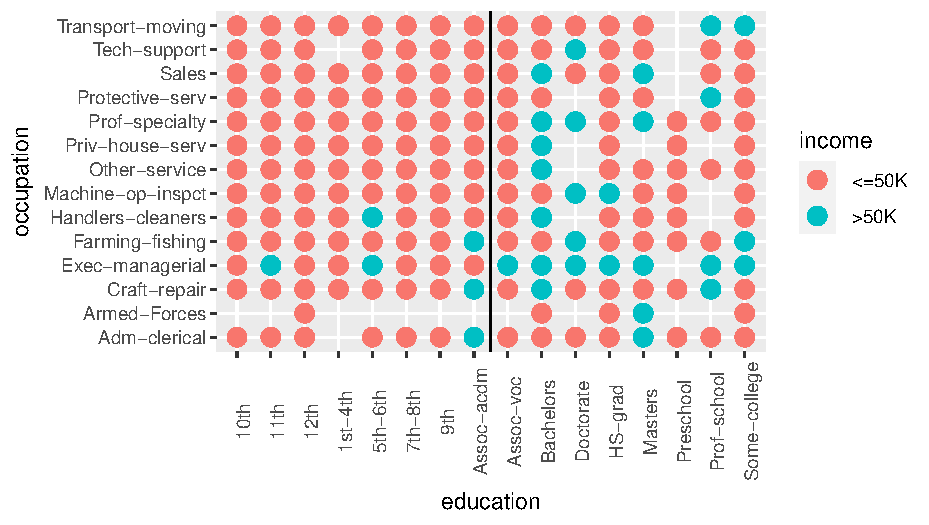
\includegraphics{MJ_Ribeiro_files/figure-beamer/unnamed-chunk-22-1.pdf}

\end{frame}

\begin{frame}[fragile]{Inductor to categorical dependet variables}
\protect\hypertarget{inductor-to-categorical-dependet-variables-2}{}

\begin{itemize}
\tightlist
\item
  I used 28000 observations to train, and 2161 to test my algorithm
\end{itemize}

\begin{Shaded}
\begin{Highlighting}[]
\NormalTok{tr1 =}\StringTok{ }\NormalTok{census[}\DecValTok{1}\OperatorTok{:}\DecValTok{28000}\NormalTok{, ]}
\NormalTok{tst1 =}\StringTok{ }\NormalTok{census[}\DecValTok{28001}\OperatorTok{:}\DecValTok{30162}\NormalTok{, ]}
\NormalTok{cl4 =}\StringTok{  }\KeywordTok{naivef}\NormalTok{(}\StringTok{'income'}\NormalTok{, tr1, }\DataTypeTok{cd=}\DecValTok{1}\NormalTok{)}
\end{Highlighting}
\end{Shaded}

\begin{verbatim}
## [1] "=-=-=-=-=-=-=-=-=-=-=-=-=-=-=-=-=-=-=-=-=-=-=-=-=-=-=-"
## [1] "Marcos Naive Bayes Classifier for Discrete Predictors"
## [1] "=-=-=-=-=-=-=-=-=-=-=-=-=-=-=-=-=-=-=-=-=-=-=-=-=-=-=-"
## A-priori probabilities:
## 
##     <=50K      >50K 
## 0.7521786 0.2478214 
## Conditional Probabilities:
\end{verbatim}

\end{frame}

\begin{frame}[fragile]{Predict}
\protect\hypertarget{predict-6}{}

\begin{itemize}
\tightlist
\item
  I used cclas = 0, so, my function return the probabilities of income
  be \textgreater50K or \textless=50k
\end{itemize}

\begin{Shaded}
\begin{Highlighting}[]
\KeywordTok{head}\NormalTok{(}\KeywordTok{predf}\NormalTok{(}\StringTok{'income'}\NormalTok{, tr1, tst1, cl4, }\DataTypeTok{cclas=}\DecValTok{0}\NormalTok{, }\DataTypeTok{cd=}\DecValTok{1}\NormalTok{))}
\end{Highlighting}
\end{Shaded}

\begin{verbatim}
##          <=50K      >50K
## [1,] 0.8195526 0.1804474
## [2,] 0.2398712 0.7601288
## [3,] 1.0000000 0.0000000
## [4,] 1.0000000 0.0000000
## [5,] 1.0000000 0.0000000
## [6,] 0.3256560 0.6743440
\end{verbatim}

\end{frame}

\begin{frame}[fragile]{Predict}
\protect\hypertarget{predict-7}{}

\begin{itemize}
\tightlist
\item
  Here I used cclas = 1, so, my function return the class the attribute
\end{itemize}

\begin{Shaded}
\begin{Highlighting}[]
\NormalTok{ndp =}\StringTok{ }\KeywordTok{predf}\NormalTok{(}\StringTok{'income'}\NormalTok{, tr1, tst1, cl4, }\DataTypeTok{cclas=}\DecValTok{1}\NormalTok{, }\DataTypeTok{cd=}\DecValTok{1}\NormalTok{)}
\KeywordTok{head}\NormalTok{(ndp)}
\end{Highlighting}
\end{Shaded}

\begin{verbatim}
## [1] " <=50K" " >50K"  " <=50K" " <=50K" " <=50K" " >50K"
\end{verbatim}

\end{frame}

\begin{frame}[fragile]{Predict}
\protect\hypertarget{predict-8}{}

\begin{itemize}
\tightlist
\item
  The acurracy of my algorithm in this case is 75.16\%
\end{itemize}

\begin{Shaded}
\begin{Highlighting}[]
\NormalTok{acurracy1 =}\StringTok{ }\NormalTok{(}\KeywordTok{sum}\NormalTok{((ndp}\OperatorTok{==}\NormalTok{tst1[,}\StringTok{'income'}\NormalTok{])}\OperatorTok{*}\DecValTok{1}\NormalTok{)}\OperatorTok{/}\KeywordTok{length}\NormalTok{(tst1[,}\DecValTok{1}\NormalTok{])) }\OperatorTok{*}\DecValTok{100}
\NormalTok{acurracy1 }
\end{Highlighting}
\end{Shaded}

\begin{verbatim}
## [1] 75.16189
\end{verbatim}

\end{frame}

\begin{frame}{Predict financial crisis using my algoritm}
\protect\hypertarget{predict-financial-crisis-using-my-algoritm}{}

\begin{itemize}
\tightlist
\item
  I want predict crisis in brasilian stock market
\item
  One of the most important models in finance is CCAPM. The complete
  derivation of the model can be view in my
  \href{https://mj-ribeiro.github.io/ecofin.pdf}{Github}
\item
  The principal equation of the model is:
\end{itemize}

\begin{equation}\label{eq12}
    E(R^i_{t+1}) - R^f_{t+1} = \lambda_{g_{t+1}} \beta_{i,g_{t+1}}
\end{equation}

where

\begin{equation}\label{eq13}
    \beta_{i,g_{t+1}} = \left(\frac{Cov_t(g_{t+1}, R_{t+1})}{Var_t(g_{t+1})} \right) 
\end{equation}

and

\begin{equation}\label{eq14}
    \lambda_{g_{t+1}} = \gamma Var_t(g_{t+1})
\end{equation}

\end{frame}

\begin{frame}{Predict financial crisis using my algoritm}
\protect\hypertarget{predict-financial-crisis-using-my-algoritm-1}{}

\begin{itemize}
\tightlist
\item
  \(R^i_{t+1}\) is the return of asset i
\item
  \(R^f_{t+1}\) is the risk free asset
\item
  The left side of the equation is known as the risk premium
\item
  \(g_{t+1}\) is the consumption growth
\item
  \(t\) is a time subscript
\item
  \(\gamma\) is the risk aversion and \(\beta\) the price of risk
\item
  I will not go into the details of the model so as not to lose the
  focus of the work
\item
  My claim is that i can predict crisis in brasilian stock market using
  risk aversion \(\gamma\)
\item
  Just create a variable that represents crisis in the stock market
  brasilian, create a proxy for risk aversion \(\gamma\), and choice
  other dependent variable
\end{itemize}

\end{frame}

\begin{frame}{Crisis proxy}
\protect\hypertarget{crisis-proxy}{}

\begin{itemize}
\tightlist
\item
  To make a crisis proxy i create CMAX algorithm to detects extreme
  price levels, in Ibovespa returns, over a given period (12 months for
  example)
\item
  CMAX equation can be see below
\end{itemize}

\begin{equation}\label{eq15}
  CMAX_t = \frac{p_t}{max(p_{t-12},\dotsb,p_t)}
\end{equation}

\end{frame}

\begin{frame}[fragile]{Crisis proxy}
\protect\hypertarget{crisis-proxy-1}{}

\begin{itemize}
\tightlist
\item
  And my CMAX algorithm is:
\end{itemize}

\begin{Shaded}
\begin{Highlighting}[]
\NormalTok{CMAX =}\StringTok{ }\ControlFlowTok{function}\NormalTok{(w, n, s)\{}
\NormalTok{  l =}\StringTok{ }\KeywordTok{matrix}\NormalTok{(}\DataTypeTok{nrow=}\NormalTok{n,}\DataTypeTok{ncol =}\NormalTok{ (w}\OperatorTok{+}\DecValTok{1}\NormalTok{))}
\NormalTok{  max =}\StringTok{ }\KeywordTok{matrix}\NormalTok{(}\DataTypeTok{nrow=}\NormalTok{n, }\DataTypeTok{ncol =} \DecValTok{1}\NormalTok{)}
\NormalTok{  cmax =}\StringTok{ }\KeywordTok{matrix}\NormalTok{(}\DataTypeTok{nrow=}\NormalTok{n, }\DataTypeTok{ncol =} \DecValTok{1}\NormalTok{)}
  \ControlFlowTok{for}\NormalTok{ (j }\ControlFlowTok{in} \DecValTok{1}\OperatorTok{:}\NormalTok{n)\{}
    
\NormalTok{    l[j, }\DecValTok{1}\OperatorTok{:}\NormalTok{(w}\OperatorTok{+}\DecValTok{1}\NormalTok{)] =}\StringTok{ }\NormalTok{s[j}\OperatorTok{:}\NormalTok{(w}\OperatorTok{+}\NormalTok{j)]}
\NormalTok{    max[j] =}\StringTok{ }\KeywordTok{max}\NormalTok{(l[j, }\DecValTok{1}\OperatorTok{:}\NormalTok{(w}\OperatorTok{+}\DecValTok{1}\NormalTok{)])}
    
\NormalTok{    cmax[j] =}\StringTok{ }\NormalTok{l[j, (w}\OperatorTok{+}\DecValTok{1}\NormalTok{)]}\OperatorTok{/}\KeywordTok{max}\NormalTok{(max[j])}
\NormalTok{  \}}
  \KeywordTok{return}\NormalTok{(cmax)}
\NormalTok{\}}
\end{Highlighting}
\end{Shaded}

\end{frame}

\begin{frame}{Crisis proxy}
\protect\hypertarget{crisis-proxy-2}{}

\begin{itemize}
\tightlist
\item
  w is the window size
\item
  n is the number of windows
\item
  s is the vector that i will pass the function
\item
  If the CMAX exceeds a certain limit, we can say that it is a crisis
  period and the crisis proxy will be equal to 1. Otherwise, it will be
  zero
\item
  This limit can be the Value at Risk in 5\%
\end{itemize}

\end{frame}

\begin{frame}{Ibovespa returns}
\protect\hypertarget{ibovespa-returns}{}

\begin{itemize}
\tightlist
\item
  Note the big drop of ibov in 2020 in the figure (a) below. The
  vertical line in figure (b) is the limit used to define crisis. This
  is the quantile of 0.05 of Ibovespa returns. This approach is known as
  Value at Risk (Var)
  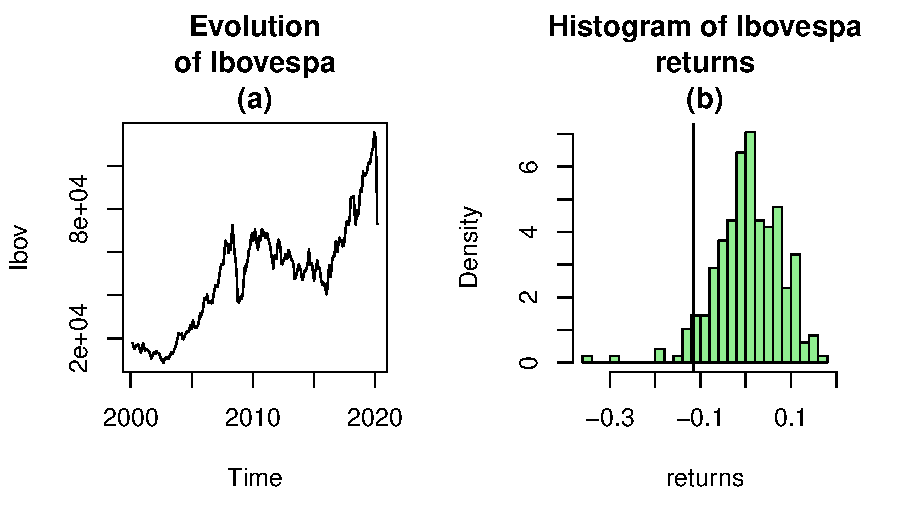
\includegraphics{MJ_Ribeiro_files/figure-beamer/unnamed-chunk-28-1.pdf}
\end{itemize}

\end{frame}

\begin{frame}{Non-categorical dependent variables}
\protect\hypertarget{non-categorical-dependent-variables}{}

\begin{itemize}
\tightlist
\item
  The other two variables that i choose is PCA and oil price
\item
  PCA was constructed using Principal Component Analysis of return of 23
  assets that compose Ibovespa index. The construction of this variable
  can be view in my
  \href{https://github.com/mj-ribeiro/College-works/blob/master/eco_fin/pca_risk_ecofin.R}{Github}
\item
  Oil price i get in Yahoo finance using quantmod library
\item
  My data is a monthly time series from 2000-03 to 2020-03
\item
  I use the data 2000-03 to 2019-05 to train model. And 2019-06 to
  2020-03 to test model
\item
  This last time interval cover COVID-19 pandemic. During this pandemic
  (2020-01 to 2020-03) the Ibovespa fell sharply
\end{itemize}

\end{frame}

\begin{frame}{Plots}
\protect\hypertarget{plots-3}{}

\begin{itemize}
\tightlist
\item
  We can see in the data that there is no obvious pattern that allows
  the prediction of falls in the Brazilian stock market. But it seems
  that the stock market falls are associated with lower oil prices
\end{itemize}

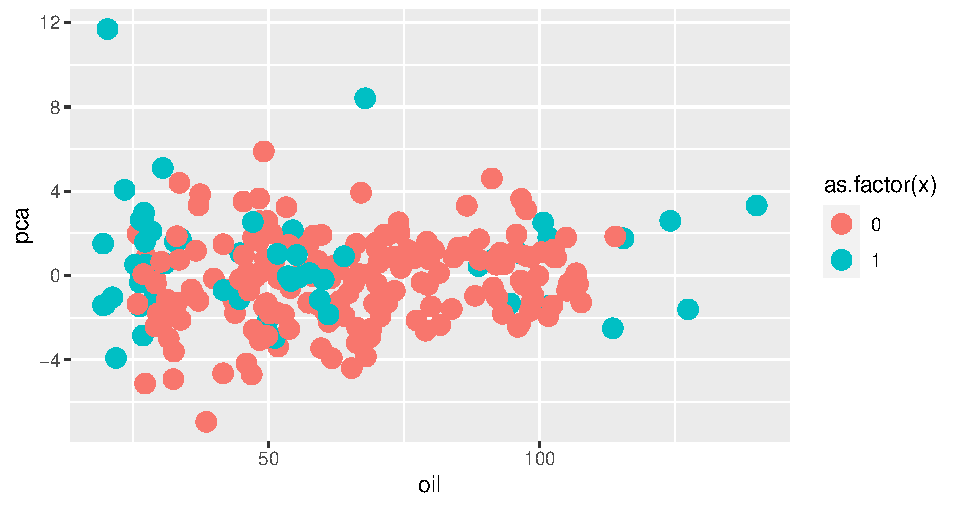
\includegraphics{MJ_Ribeiro_files/figure-beamer/unnamed-chunk-29-1.pdf}

\end{frame}

\begin{frame}[fragile]{Inductor to crisis forecast in brasilian stock
market}
\protect\hypertarget{inductor-to-crisis-forecast-in-brasilian-stock-market}{}

\begin{itemize}
\tightlist
\item
  So, i used naivef function in my dataset
\end{itemize}

\begin{Shaded}
\begin{Highlighting}[]
\NormalTok{tr =}\StringTok{ }\NormalTok{find2[}\DecValTok{1}\OperatorTok{:}\DecValTok{231}\NormalTok{, ]}
\NormalTok{tst =}\StringTok{ }\NormalTok{find2[}\DecValTok{232}\OperatorTok{:}\DecValTok{241}\NormalTok{, ]}
\NormalTok{cl3 =}\StringTok{ }\KeywordTok{naivef}\NormalTok{(}\StringTok{'x'}\NormalTok{,tr, }\DataTypeTok{cd=}\DecValTok{0}\NormalTok{)}
\end{Highlighting}
\end{Shaded}

\begin{verbatim}
## [1] "=-=-=-=-=-=-=-=-=-=-=-=-=-=-=-=-=-=-=-=-=-=-=-=-=-=-=-"
## [1] "Marcos Naive Bayes Classifier for Discrete Predictors"
## [1] "=-=-=-=-=-=-=-=-=-=-=-=-=-=-=-=-=-=-=-=-=-=-=-=-=-=-=-"
## A-priori probabilities:
## 
##         0         1 
## 0.7965368 0.2034632
\end{verbatim}

\end{frame}

\begin{frame}[fragile]{Predict}
\protect\hypertarget{predict-9}{}

\begin{itemize}
\tightlist
\item
  I used predf funtion to predict crisis
\item
  I used cclas = 0, so, my function return the probabilities of crisis
  (x=1)
\end{itemize}

\begin{Shaded}
\begin{Highlighting}[]
\KeywordTok{predf}\NormalTok{(}\StringTok{'x'}\NormalTok{, tr, tst, cl3, }\DataTypeTok{cclas=}\DecValTok{0}\NormalTok{, }\DataTypeTok{cd=}\DecValTok{0}\NormalTok{)}
\end{Highlighting}
\end{Shaded}

\begin{verbatim}
##                  0         1
##  [1,] 6.593307e-45 1.0000000
##  [2,] 2.914477e-42 1.0000000
##  [3,] 4.459197e-39 1.0000000
##  [4,] 7.096824e-38 1.0000000
##  [5,] 1.143163e-37 1.0000000
##  [6,] 1.204856e-39 1.0000000
##  [7,] 3.048610e-47 1.0000000
##  [8,] 1.431212e-34 1.0000000
##  [9,] 3.424599e-29 1.0000000
## [10,] 5.420900e-07 0.9999995
\end{verbatim}

\end{frame}

\begin{frame}[fragile]{Predict}
\protect\hypertarget{predict-10}{}

\begin{itemize}
\tightlist
\item
  Here I used cclas = 1, so, my function return the class the attribute
\end{itemize}

\begin{Shaded}
\begin{Highlighting}[]
\KeywordTok{predf}\NormalTok{(}\StringTok{'x'}\NormalTok{, tr, tst, cl3, }\DataTypeTok{cclas=}\DecValTok{1}\NormalTok{, }\DataTypeTok{cd=}\DecValTok{0}\NormalTok{)}
\end{Highlighting}
\end{Shaded}

\begin{verbatim}
##       [,1]
##  [1,] "1" 
##  [2,] "1" 
##  [3,] "1" 
##  [4,] "1" 
##  [5,] "1" 
##  [6,] "1" 
##  [7,] "1" 
##  [8,] "1" 
##  [9,] "1" 
## [10,] "1"
\end{verbatim}

\end{frame}

\begin{frame}[fragile]{Predict}
\protect\hypertarget{predict-11}{}

\begin{itemize}
\tightlist
\item
  The accuracy of my model is 100\%
\end{itemize}

\begin{Shaded}
\begin{Highlighting}[]
\NormalTok{prev =}\StringTok{ }\KeywordTok{predf}\NormalTok{(}\StringTok{'x'}\NormalTok{, tr, tst, cl3, }\DataTypeTok{cclas=}\DecValTok{1}\NormalTok{, }\DataTypeTok{cd=}\DecValTok{0}\NormalTok{)}
\NormalTok{accuracy =}\StringTok{ }\NormalTok{(}\KeywordTok{sum}\NormalTok{((prev }\OperatorTok{==}\StringTok{ }\NormalTok{tst[,}\DecValTok{1}\NormalTok{])}\OperatorTok{*}\DecValTok{1}\NormalTok{)}\OperatorTok{/}\KeywordTok{length}\NormalTok{(tst[,}\DecValTok{1}\NormalTok{]) )}\OperatorTok{*}\DecValTok{100}
\NormalTok{accuracy}
\end{Highlighting}
\end{Shaded}

\begin{verbatim}
## [1] 100
\end{verbatim}

\begin{itemize}
\tightlist
\item
  This accuracy may have been caused by the fact that the fall in the
  Brazilian stock market was very sharp
\end{itemize}

\end{frame}

\begin{frame}{}
\protect\hypertarget{section}{}

\begin{center}
  \huge{Thanks!}
\end{center}

\end{frame}

\end{document}
